\section{Ecology, open-endedness, and experimental measurement}
\subsection{Space changes mechanisms, not only appearance}
Spatial organization can alter which interactions reproduce. Hypercycle and
replicator models demonstrate that waves and restricted mixing can protect
some productive organizations against exploitation
\citep{Boerlijst1991,Takeuchi2009}. Their catalytic relationships are prescribed,
so they do not establish that an instruction-level VM will generate the same
ecology. They do show why a well-mixed comparison and a spatial model can
select differently even when both sustain a population.

For executable systems, the corresponding hypothesis must be expressed in
operations: where a program can read, where copying reserves space, which
neighbors can exploit instructions, and how opportunities move across the
grid. A selected snapshot of a wave is insufficient. Measurements should
include invasion failure, extinction, spatial correlations, available space,
and the work spent on successful and unsuccessful reproduction.

\subsection{Scheduling and the meaning of reproducibility}
Update order is part of a dynamical model. The partially accessible study by
Sch\"onfisch and de Roos distinguishes several asynchronous procedures and
reports effects of update-order correlations \citep{Schonfisch1999}. Its
publisher preview supports the need to specify the algorithm; it is not used
here as a proof about a stochastic allocating VM. A fresh random permutation,
sampling sites with replacement, and event-driven waiting times are different
processes.

For a two-phase digital model, the transition can be described schematically as
\begin{align}
 I_t &= E(S_t;\theta,\xi_t),\\
 S_{t+1} &= R(S_t,I_t;\theta,\xi_t),
\end{align}
where $S_t$ is the full state, $I_t$ the proposed effects, $\theta$ the rule
configuration, and $\xi_t$ the designated random inputs. This is a conceptual
decomposition, not a complete TIDE specification. Read visibility, conflict
priority, reservation release, and newborn activation still require explicit
definitions.

Counter-based random generators can associate draws with logical events
instead of an order-dependent stream \citep{Salmon2011}. That supports replay
across execution partitions, but does not supply the event-identity mapping
or make ambiguous transitions deterministic. Reproducing identical state
hashes across implementations of one rule is a different claim from finding
similar ecological outcomes under different rules. Equal seeds do not make
synchronous and sequential models equivalent.

\begin{figure}[!htbp]
\centering
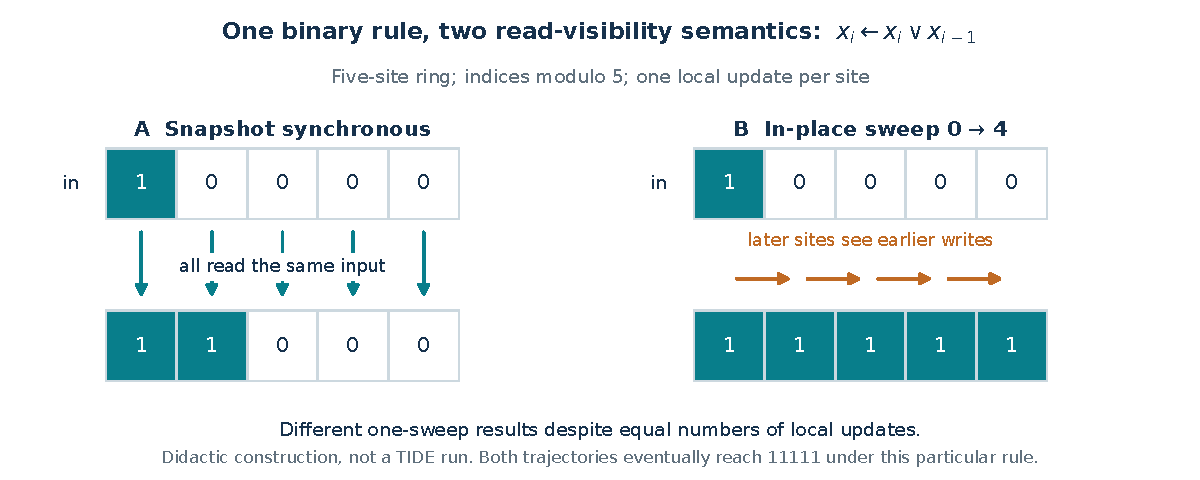
\includegraphics[width=\textwidth]{figures/update-semantics.pdf}
\caption{An original deterministic example of read visibility. With periodic
boundaries, $x_i\leftarrow x_i\lor x_{i-1}$ and initial state $10000$, one
snapshot-synchronous update yields $11000$; an in-place sweep in order
$0,1,2,3,4$ yields $11111$. Both perform five local evaluations. This constructed
example illustrates the scheduling distinction discussed above, not an
experiment from the cited literature or TIDE. Both eventually saturate under
this particular rule, so the immediate difference does not establish a
long-term ecological effect.}
\label{fig:scheduling}
\end{figure}
The finite example in Figure~\ref{fig:scheduling} isolates read visibility
without adding resource or mutation differences.

\subsection{Stagnation and functional change}
Program length, diversity, and complexity can move independently. Standish's
Tierra studies include size growth without growth in the measured complexity,
and a parsimony sweep whose limited improvements did not establish
open-endedness \citep{Standish2003,Standish2004}. A plateau therefore needs a
specified observable and observation horizon. Extinction is a separate outcome
from a surviving population whose reproductive behavior stops changing.

Responsive ecological feedback is one possible source of changing selective
conditions. Zaman and colleagues use frozen and replayed parasite controls to
distinguish responsive coevolution from exposure to a fixed collection of
opponents \citep{Zaman2014}. Their Avida setting defines infection and a suite
of logic tasks. The causal control is informative; the task-based complexity
measure and interaction rules do not transfer unchanged to task-free digital
ecology. Likewise, Chromaria's preliminary opportunity-creation ablation
motivates a hypothesis, not a universal necessity theorem
\citep{Soros2014}. Access to that paper in this review was limited to indexed
primary-text passages.

\subsection{Measure several properties instead of declaring a binary victory}
The open-ended-evolution workshop synthesis separates observable hallmarks
from proposed enabling mechanisms \citep{Taylor2016}. MODES develops
operational diagnostics for change, novelty, complexity, and ecology
\citep{Dolson2019}. Its filtering and component definitions are choices that
must remain visible. Persistence can help distinguish fleeting variation from
longer-lived contributions, but it does not exclude all drift. An informative
site count is context-dependent and can miss interactions among sites.

\begin{table}[htbp]
\centering\small
\caption{A measurement panel for soft artificial life. These are review
recommendations, not an approved event schema or a new fitness function.}
\begin{tabularx}{\textwidth}{@{}>{\raggedright\arraybackslash}p{28mm}YY@{}}
\toprule
Property & Observable example & Essential qualification \\
\midrule
Reproduction & Products and repeated viable descendants in replay & One copied fragment need not reproduce \\
Persistence & Descendants after declared lags; survival curves & Drift and spatial isolation can preserve lineages \\
Novelty & First observed behavioral signatures, separately from new byte strings & Recurrence and neutral variation can inflate turnover \\
Complexity & Contextual perturbation effects alongside program length & Length, indispensable sites and algorithmic complexity differ \\
Interaction & Focal reproduction alone, paired, and under controlled substitutions & Pair tests can miss higher-order or density-dependent effects \\
Spatial ecology & Invasion, wave persistence, spatial correlations and extinctions & A visually organized survivor can be an unrepresentative run \\
\bottomrule
\end{tabularx}
\label{tab:measurement}
\end{table}

At least three denominators should be considered when comparing treatments:
world steps, executed instructions, and occupied or available resources.
If two schedulers provide different work per step, equal step counts are not
equal computational exposure. If one treatment contains more organisms, more
new genotypes may simply reflect more reproductive events. Normalization
should answer a declared question, while retaining the raw observations.

Finite observation also creates censoring. A lineage born near the end of a
run has not had the same opportunity to pass a persistence threshold as an
early lineage. Its classification is unresolved, rather than automatically
unsuccessful. Genotype archives should include extinct variants, and sampling
limits should disclose which short-lived events can be missed.

\begin{figure}[!htbp]
\centering
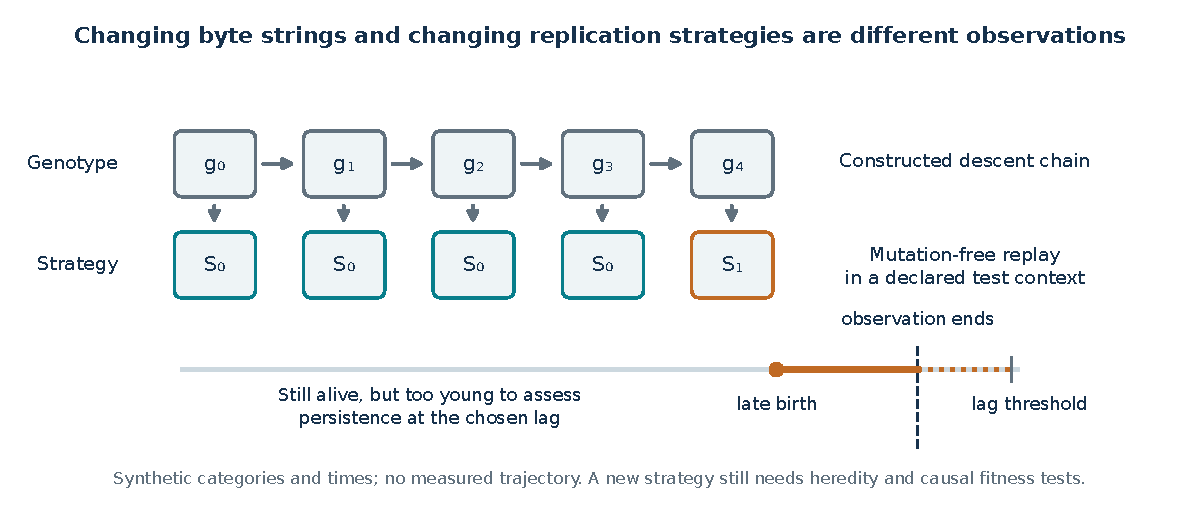
\includegraphics[width=\textwidth]{figures/measurement-limits.pdf}
\caption{Original categorical illustrations of two measurement limits.
Distinct genotypes can be equivalent under a declared mutation-free test
panel; a newly distinguished strategy still needs heredity and causal
reproductive-effect tests. This distinction is motivated by
\citet{Standish2003,Taylor2016}. The separate lower timeline shows a lineage
alive at observation cutoff but younger than the persistence lag; its status
at that lag is unresolved. The dotted future segment is unobserved, not
continued survival. Categories and times are constructed, not measured data.}
\label{fig:measurement}
\end{figure}
Figure~\ref{fig:measurement} separates observable genotype change, operational
strategy change, and incomplete follow-up.

\subsection{From description to causal evidence}
An analysis label should follow a controlled comparison. One useful design
compares A alone, B alone, and A+B under specified placement, duration,
permissions, and resource conditions. Further substitutions can disable an
instruction source, replace copied data, or alter whether a neighbor responds.
The goal is to locate the causal dependency, not to preserve a preferred
ecological classification.

Such tests also reveal the limits of static genome analysis. The same bytes
can support different outcomes in different contexts, while distinct genomes
can implement similar reproductive behavior. Functional equivalence must
therefore be defined relative to a test panel and reported at that resolution.
An empirical claim of innovation should identify the newly expressed behavior,
its heredity, its persistence, and its reproductive consequences. No finite
run establishes indefinite innovation, and a bounded fixed-state system has
only finitely many distinct states. Scale extension and sensitivity analysis
strengthen a finite claim without turning it into a proof of unboundedness.
